
\chapter{Resolución del trabajo}
 
Este capítulo está dividido en cuatro subapartados, en los que se describen las características de la Familia Zynq-7000, así 
como su arquitectura, la tarjeta usada (ZYBO) junto con sus características. Además se realiza la descripción de la plataforma Vivado y se explican las 
distintas etapas del flujo de diseño y los módulos hardware que se van a usar, un procesador, una memoria RAM, un módulo de generación de reloj y 
un controlador VGA. Por último se realizan un par de casos prácticos haciendo uso de los módulos explicados en las secciones anteriores. 

\section{Materiales}

En esta sección se describen los principales materiales usados en este proyecto dividiéndola en 3 apartados, la familia Zynq-7000 junto a sus 
características, la tarjeta Zybo y sus especificaciones y la herramienta Vivado.

\subsection{Familia Zynq-7000}

La familia \textbf{Zynq-7000} se basa en la arquitectura SoC. Estos productos integran un sistema de procesamiento basado en \textit{ARM Cortex-A9} 
de un sólo núcleo o dual-core con muchas funciones y lógica programable de 28nm. También incluye memoria ``on-chip'', interfaces de memoria externa e 
interfaces de conectividad periféricas \cite{zynq7000}.

Esta familia ofrece la flexibilidad y escalabilidad de un FPGA, al mismo tiempo que proporciona rendimiento, potencia y facilidad de uso típicamente 
asociados con ASIC y ASSP. Su gama de dispositivos permite crear aplicaciones de alto rendimiento. Si bien cada dispositivo de la familia Zynq-7000 
contiene el mismo sistema de procesamiento, los recursos de lógica programable y E/S varían entre los dispositivos.

La arquitectura Zynq-7000 (Ver Figura \ref{zynq-7000}) permite la implementación de lógica personalizada para configurar módulos hardware específicos 
en el PL (``Programmable Logic'') y software personalizado en el PS (``Processing System''). La integración del PS con el PL 
permite niveles de rendimiento que las soluciones de dos chips (por ejemplo, un ASSP con un FPGA) no pueden igualar debido a su ancho de banda de E/S, 
latencia y presupuestos de energía limitados.

Xilinx ofrece una gran cantidad de módulos IP (``\textit{Intellectual Property}'') para la familia Zynq-7000. Los controladores de dispositivos ``Stand-alone'' y Linux están disponibles para los 
periféricos en el PS y el PL. El entorno de desarrollo de Vivado Design Suite permite un rápido desarrollo de productos para ingenieros de software, 
hardware y sistemas. La adopción del PS basado en ARM conlleva una amplia gama de herramientas de terceros y proveedores de módulos IP.

La inclusión de un procesador de aplicaciones permite el soporte del sistema operativo de alto nivel, por ejemplo, Linux. El PS y el PL están en dominios 
de energía separados, lo que permite apagar el PL para administrar la energía. Los procesadores de la PS siempre se inician primero, permitinedo un enfoque 
centrado en el software para la configuración de PL. La configuración de PL se gestiona mediante software que se ejecuta en la CPU.

\begin{figure}
    \centering
    \includegraphics[width = 1\textwidth]{imagenes/arqfamiliazynq.png}
    \caption{\textit{Arquitectura Zynq-7000 \cite{zynq7000}}}\label{zynq-7000}
\end{figure}

La PS está dividida en cuatro bloques principales:

\begin{itemize}
    \item \textbf{APU (Unidad de Procesamiento de Aplicaciones)} - Incluye un procesador dual-core o single-core ARM Cortex-A9 MPCores, canales DMA, interruptores y relojes, entre otros.
    \item \textbf{Interfaces de Memoria} - Incluye módulos de controladores de memoria dinámica (DDR3) e interfaces de memoria estática (por ejemplo, interfaz flash NAND).
    \item \textbf{IOP (Periféricos E/S)} - Esta unidad contiene los periféricos de comunicación de datos (USB, Ethernet MAC, por ejemplo).
    \item \textbf{Interconexiones} - Los tres anteriores están todos conectados entre sí y al PL a través de una interconexión ARM AMBA AXI de varias capas.
\end{itemize}

El PL incluye:

\begin{itemize}
    \item \textbf{CLB} - Incluye LUT que se puede configurar como una LUT de 6 entradas con una salida, o como dos de 5 entradas con salidas independientes. 
    Cada salida LUT se puede registrar en un flip-flop. Estos CLBs están formados por dos segmentos, que están constituidos por cuatro de estos LUT y 8 flip-flops, así como 
    los multiplexores y la lógica aritmética.
    \item \textbf{Bloque RAM} - Incluye ``dual-port'', lógica FIFO programable y circuito integrado opcional de corrección de errores.
    \item \textbf{Bloques DSP (``Digital Signal Processing'')} - Cada segmento de DSP consiste en un multiplicador de complemento a dos y un acumulador de 48 bits. Incluye un 
    pre-sumador adicional. Este pre-sumador mejora el rendimiento. El DSP también incluye un detector de patrones que se puede utilizar para redondeo.
    \item \textbf{Bloques E/S Programables}
    \item \textbf{Módulo de configuración PL}
\end{itemize}

La arquitectura Zynq AP SoC (XC7Z010-1CLG400C) incluida en la tarjeta Zybo está dividida también en dos partes (Figura \ref{zynq-7000}), el (\textit{PS}) y la (\textit{PL}). 
La PL usada es parecida a la de la FPGA \textit{Xilinx 7-series Artix}, excepto porque contiene buses y puertos dedicados que hacen que esté 
acoplado fuertemente al PS. Contiene 28K de celdas lógicas programables, 17.600 LUTs, 35.200 Flip-Flops, 2.1Mb de bloque RAM y 80 bloques DSP. Además, 
cada dispositivo de la familia Zynq-7000 tiene hasta 8 ``clock management tiles'' (CMTs) que son un conjunto de MMCM y PLL. En concreto, esta arquitectura tiene 2 MMCM 
y 2 PLL.

El PS consiste en un conjunto de componentes como la \textit{APU} (Unidad de Procesamiento de Aplicaciones) que incluye dos procesadores ARM Cortex-A9 MPCore, 
\textit{AMBA} (Arquitectura de Bus de Microcontrolador Avanzada), Controlador de Memoria \textit{DDR3}, y varios controladores periféricos con 
las entradas y salidas multiplexadas a 54 pines dedicados (\textit{MIO}). Los controladores periféricos están conectados al procesador mediante 
la interconexión \textit{AMBA} y la PL está conectada de la misma manera.

\subsection{Tarjeta Zybo}

La FPGA de la familia Zynq 7000 descrita en la sección anterior es incluida en tarjeta \textbf{ZYBO} (\textit{ZYbo BOard}) \cite{manual_zybo}. Es una plataforma de desarrollo de circuito 
digital, y está construida alrededor del miembro más pequeño de la familia Zynq-7000, el \textbf{Z-7010}, que se basa en la arquitectura 
\textbf{AP SoC} (\textit{Xilinx All Programmable System-on-Chip}), que integra un procesador de doble núcleo ARM Cortex-A9 con lógica \textit{Xilinx 7-series FPGA}.

La tarjeta Zybo ofrece las siguientes caraterísticas (Figura \ref{fig:zybo}):

\begin{itemize}
    \item ZYNQ XC7Z010-1CLG400C
    \item Puerto HDMI de doble función (fuente/receptor)
    \item Puerto VGA de 16 bits por pixel
    \item Ethernet PHY trimodo (1Gbit/100Mbit/10Mbit)
    \item MicroSD
    \item OTG USB 2.0 PHY
    \item EEPROM externo
    \item Códec de audio con salida de auricular y micrófono 
    \item 128Mb Serial Flash con interfaz QSPI
    \item Programación JTAG ``on-board'' y convertidor UART a USB
    \item GPIO: 6 botones, 4 interruptores, 5 LEDs
    \item 6 conectores Pmod (1 procesador dedicado, 1 dual analógico / digital, 3 diferenciales de alta velocidad, 1 lógico dedicado)
    \item Procesador dual-core Cortex-A9 de 650Mhz
    \item Controlador de memoria DDR3 con 8 canales DMA
    \item Controladores periféricos de alto ancho de banda: 1G Ethernet, USB 2.0, SDIO
    \item Controladores periféricos de bajo ancho de banda: SPI, UART, CAN, \(I^2C\)
    \item Lógica Reprogramable equivalente a Artix-7 FPGA
\end{itemize}

\begin{figure}[H]
    \centering
    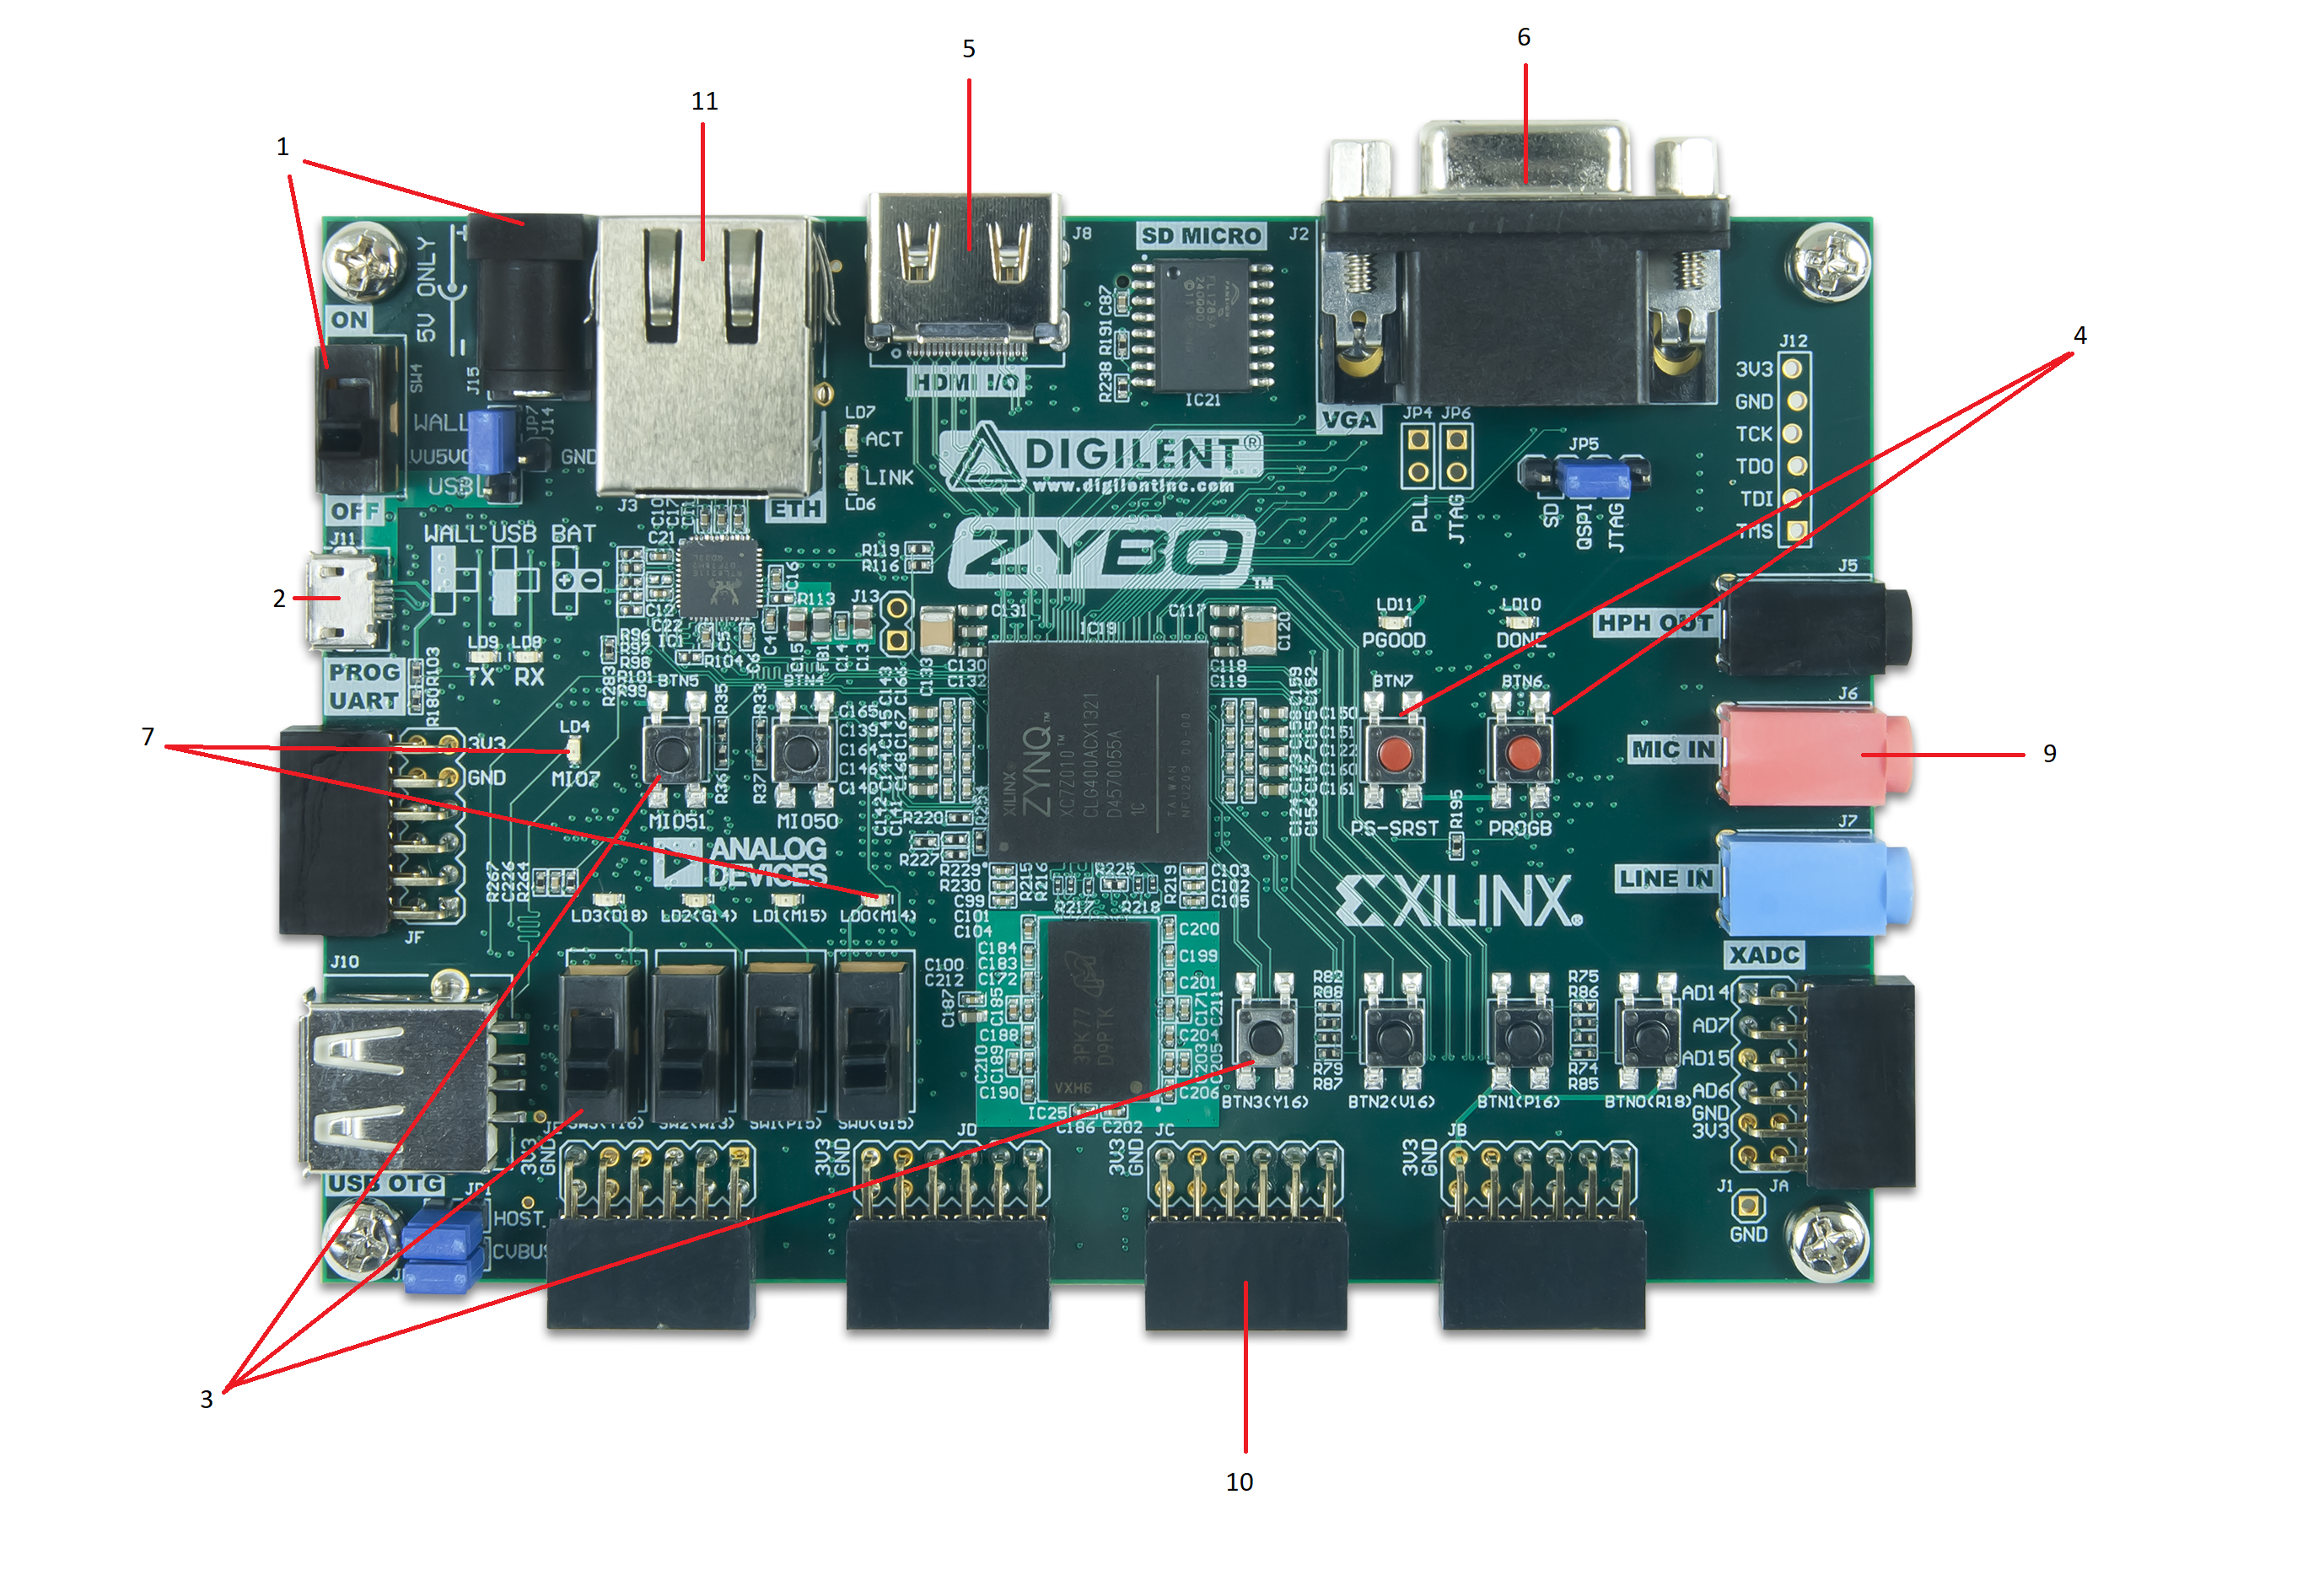
\includegraphics[width = 1\textwidth]{imagenes/zybo2.png}
    \caption{\textit{ZYBO Zynq-7000 Development Board \cite{manual_zybo}}}\label{fig:zybo}
\end{figure}

La tarjeta Zybo incluye cuatro interruptores, cuatro botones y cuatro LEDs individuales a la PL. Además hay 2 botones y un LED conectados 
directamente al PS a través de pines MIO. Adicionalmente hay un LED de encendido de la tarjeta, otros dos para el estado del puerto USB 
y un último LED para el estado de la programación de la FPGA.

Uno de los \textbf{botones de reset} reestablece la PL, que permanecerá sin configurar hasta ser reprogramado de nuevo. El otro reinicia 
el dispositivo sin afectar al entorno de depuración. 

Nos encontramos con tres \textbf{Conectores de audio}, dos entradas para micrófono y línea estéreo y una salida para auriculares.

El \textbf{Puerto VGA} (\textit{Video Graphics Array}) es una interfaz que envía una señal desde la FPGA al conector VGA. Éste se suele usar 
para conectar dispositivos. La placa ZYBO utiliza 18 pines lógicos programables para crear un puerto de salida VGA analógico. Esto se traduce 
en una profundidad de color de 16 bits (5 bits para el rojo, 6 para el verde y 5 para el azul) y dos señales de sincronización estándar. La 
conversión de digital a analógico se realiza utilizando una  escalera de resistencia R-2R simple. La escalera trabaja en conjunto con la resistencia 
de terminación de 75 ohmios de la pantalla VGA para crear señales VGA rojas, azules y verdes de 32 y 64 niveles de señal analógica.

En la sección 5.3 se realizará una descripción de este componente para más tarde usarlo en un caso práctico de la sección 5.4.

El \textbf{Puerto HDMI} es un conector de entrada y salida con el que se puede transmitir vídeo compatible con HDMI o DVI. 

Los \textbf{Conectores Pmod} (\textit{Módulos Periféricos}) son unos conectores con estándares de módulos periféricos, para ampliar la capacidad de la 
lógica programable. Se comunican mediante 6,8 ó 12 pines para transportar señales de control digital. En nuestro caso, son 12 pines (2x6). 
Hay 6 conectores Pmod con distinto comportamiento en esta tarjeta y cada uno pertenece a una de las cuatro categorías, ``standard'', ``MIO connected'', 
``XADC'' y ``high-speed''. Por ejemplo, la conexión PS2 para conectar teclados y ratones, podría ser un buen ejemplo para realizar algún ejercico práctico 
con propósito académico.

\subsection{Vivado}

El software de Xilinx \textbf{ISE} no estaba preparado para soportar la complejidad y capacidad de un diseño de una FPGA con un procesador 
ARM. \textit{Vivado Design Suite} (Figura \ref{vivadoGUI}) fue desarrollado para FPGAs con más capacidad y permite compilaciones de descripciones 
basadas en \(C\) gracias a la funcionalidad de síntesis de alto nivel.

Zybo es compatible con \textit{Vivado Design Suite} así como con el conjunto de herramientas ISE/EDK.
Estas herramientas combinan el diseño lógico FPGA con el desarrollo software de ARM. Se pueden utilizar para diseñar sistemas 
de cualquier complejidad, desde un sistema operativo completo hasta un programa simple que controla algunos LEDs.

\textbf{Vivado Design Suite} es un entorno de diseño integrado (\textbf{IDE}) de Xilinx para la síntesis y análisis de diseños HDL. Vivado incluye 
su propio simulador lógico y además está la posibilidad de usar otros simuladores como \textit{ModelSim}, \textit{Mentor Questa}, 
\textit{Candence IES} o \textit{Synopsys VCS}. Además incluye síntesis a alto nivel con una herramienta que convierte código C a lógica
 programable.

Está formado por 4 componentes:
\begin{itemize}
    \item \textbf{Vivado High-Level Synthesis} - Permite usar programas en \(C\), \(C++\) y \(SystemC\) en dispositivos Xilinx  sin necesidad 
    de crear un RTL manualmente. Aumenta la productividad del desarrollador y admite clases, plantillas, funciones y sobrecarga de operadores.
    \item \textbf{Vivado Simulator} - Es un simulador controlado por eventos de lenguaje de descripción hardware (\textbf{HLD}) que admite 
    simulación de comportamiento y tiempos. Además admite scripts TCL (\textit{Tool Command Language}) en lenguaje mixto, es decir, admite
     lenguajes como \textit{Verilog}, \textit{SystemVerilog} y \textit{VHDL}.
    \item \textbf{Vivavo IP Integrator} - Permite integrar y  configurar IP (``\textit{Intellectual Property}") desde la biblioteca propia de Xilinx.
    \item \textbf{Vivado TCL Store} - Es un sistema de comandos para desarrollar complementos para Vivado además de agregar y modificar las 
    capacidades de Vivado. Todas las funciones de Vivado se pueden controlar con los scripts TCL.
\end{itemize}

En concreto, la versión que se ha utilizado es con Vivado 2020.1. Para trabajar con él, se puede hacer tanto trabajando con la TCL o 
directamente con la GUI de Vivado IDE \cite{vivadoIDE}. 
\begin{figure}[H]
    \centering
    \includegraphics[width = 1\textwidth]{imagenes/Vivado1.png}
    \caption{\textit{Vivado IDE}}\label{vivadoGUI}
\end{figure}

La sección \textbf{Quick Start} nos proporciona fácil acceso a la creación de un nuevo proyecto, abrir proyectos existentes o abrir proyectos 
de ejemplo ofrecidos por Xilinx. Además, en la sección \textbf{Recent Projects} se pueden abrir proyectos usados recientemente.

En la sección \textbf{Tasks} encontramos el acceso a \textbf{Manage IP} que nos permite ver el catálogo de módulos IP, personalizar módulos IP y generar 
productos de salida.  \textbf{Open Hardware Manager} nos permite conectar la tarjeta y descargar un programa en el dispositivo FPGA. 
\textbf{XHub Store} sirva para instalar placas, aplicaciones Tcl (de código abierto) y diseños de ejemplo desarrollados por Xilinx y otros proveedores. 

La última sección es \textbf{Learning Centre} donde se encuentra el acceso directo a la documentación, tutoriales y videos sobre lo que se 
puede hacer con esta herramienta.

Los componentes principales del entorno principal de Vivado (ver Figura \ref{vivado2} son:
\begin{enumerate}
    \item \textit{Menu Bar}
    \item \textit{Main Toolbar}
    \item \textit{Flow Navigator}
    \item \textit{Layout Selector}
    \item \textit{Data Windows Area}
    \item \textit{Workspace} 
    \item \textit{Menu Command Search Field} 
    \item \textit{Project Status Bar} 
    \item \textit{Results Windows Area}
\end{enumerate}

\begin{figure}[H]
    \centering
    \includegraphics[width = 1\textwidth]{imagenes/vivado2.png}
    \caption{\textit{Entorno Principal Vivado IDE}}\label{vivado2}
\end{figure}

\textit{Flow Navigator} (Figura \ref{flownavigator}) permite acceder a comandos y herramientas que van desde abrir diseños a crear un archivo bitstream. Las 
diferentes secciones permiten hacer lo siguiente:
\begin{itemize}
    \item \textit{\textbf{Project Manager}}: Cambio de ajustes generales, añadir o crear archivos o abrir el Catálogo de IPs
    \item \textit{\textbf{IP Integrator}}: Crear, abrir o generar un bloque de diseño. 
    \item \textit{\textbf{Simulation}}: Ejecutar una simulación
    \item \textit{\textbf{RTL Analysis}}: Abrir un diseño elaborado o generar un diseño de diagrama de circuitos RTL.
    \item \textit{\textbf{Synthesis}}: Ejecutar la síntesis o abrir el diseño sintetizado, donde se encuentran informes sobre el mismo que realiza Vivado.
    \item \textit{\textbf{Implementation}}: Ejecutar la implementación, implementar un disñeo activo o abrir el diseño implementado, donde se encuentran informes sobre el mismo que realiza Vivado.
    \item \textit{\textbf{Program and Debug}}: Generar un archivo bitstream o abrir una ventana para conectar la tarjeta FPGA y programarla.
\end{itemize}

\begin{figure}[H]
    \centering
    \includegraphics[width = 0.3\textwidth]{imagenes/flownavigator.png}
    \caption{\textit{Flow Navigator}}\label{flownavigator}
\end{figure}

\textit{Layout Selector} proporciona el diseño de ventanas predefinidas para facilitar el proceso de diseño. Entre las opciones tenemos:
\begin{itemize}
    \item \textit{\textbf{Default Layout}}: Muestra el diseño con el mínimo número de ventanas, con un resumen global del diseño (Figura \ref{default}).
    \item \textit{\textbf{I/O Planning}}: Definición de restricciones de ubicación I/O y colocación de puertos (Figura \ref{io}).
    \item \textit{\textbf{Floorplanning}}: Gestionar particiones y tareas jerárquicas (Figura \ref{fp}).
    \item \textit{\textbf{Timing Analysis}}: Ejecutar informes de tiempo y analizarlo (Figura \ref{ta}).
\end{itemize} 

\begin{figure}[H]
    \centering
    \includegraphics[width = 0.7\textwidth]{imagenes/default.png}
    \caption{\textit{Default Layout}}\label{default}
\end{figure}

\begin{figure}[H]
    \centering
    \includegraphics[width = 1\textwidth]{imagenes/io.png}
    \caption{\textit{I/O Planning}}\label{io}
\end{figure}

\begin{figure}[H]
    \centering
    \includegraphics[width = 1\textwidth]{imagenes/fp.png}
    \caption{\textit{Floorplanning}}\label{fp}
\end{figure}

\begin{figure}[H]
    \centering
    \includegraphics[width = 1\textwidth]{imagenes/ta.png}
    \caption{\textit{Timing Analysis}}\label{ta}
\end{figure}

\textit{Project Status Bar} da información sobre el estado actual del diseño activo. \textit{Data Windows Area} muestra información 
sobre los archivos que forman el diseño. \textit{Workspace} muestra ventanas como el editor de textos o el diseño del diagrama de 
circuitos, entre otros. Y \textit{Results Windows Area} presenta los resultados de los comandos ejecutados. Además se muestran 
distintas ventanas, como \textit{Tcl Console}, \textit{Messages}, \textit{Log}, \textit{Reports} y \textit{Design Runs}.

\section{Metodología}

Para el desarrollo de este trabajo se ha seguido una planificación y secuencia temporal concreta. Primero se ha revisado el estado actual 
del mercado de FPGAs, centrándonos en los dispositivos y herramientas software del fabricante Xilinx (apartado 1.3). Después, se han estudiado las 
características de la tarjeta y se han realizado algunas pruebas de configuración como encender y apagar los leds de la tarjeta. A continuación, 
se ha estudiado el flujo de diseño con Vivado para síntesis RT-lógica a partir de descripciones VHDL, en concreto, a partir de la 
documentación aportada por el fabricante (Xilinx), se ha estudiado detalladamente las diferentes funcionalidades y se han reproducido 
experimentalmente con un ejemplo sencillo. Con esto, hemos seguido el flujo de diseño para generar y validar módulos IP que han sido 
útiles para la realización de prácticas en asignaturas relacionadas con este tema. Por último se han utilizado estos módulos en dos casos 
prácticos para validarlos experimentalmente.

Dentro del flujo de diseño, lo que más ha llevado tiempo ha sido el tema de la simulación y los dos tipos de simulación funcional y temporal. Además 
me costó crear bien los testbech para poder realizar las simulaciones. La principal dificultad a la hora de realizar el trabajo ha sido tener que entender 
la metodología y el flujo de diseño a partir de descripciones RT.

En esta sección se trata de estudiar y describir cómo se realiza con Vivado la metodología propia de flujo de diseño con FPGAs a partir de
descripciones RT en VHDL.

Las etapas del flujo de diseño en FPGAs se explican en los siguientes apartados y son \cite{smith2010fpgas}:

\begin{enumerate}
    \item \textbf{Diseño}
    \item \textbf{Síntesis}
    \item \textbf{Simulación}
    \item \textbf{Implementación}
    \item \textbf{Generación Bitstream}
\end{enumerate}

Este flujo de diseño que ahora se va describir, se ha reproducido en base a un ejemplo sencillo (contador de 4 bits) descrito en el Anexo de este proyecto.

\subsection{Diseño}

Vivado soporta múltiples lenguajes de descripción hardware, entre ellos VHDL y Verilog, e incluso se pueden usar ficheros con ambos lenguajes. 
El siguiente diagrama (Ver Figura \ref{Dflow}) muestra un flujo de diseño típico con las herramientas de Xilinx.

\begin{figure}[H]
    \centering
    \includegraphics[width = 0.8\textwidth]{imagenes/flujo.png}
    \caption{\textit{Typical Xilinx FPGA Development Flow (Adaptada de \cite{smith2010fpgas})}}\label{Dflow}
\end{figure}

Para comenzar con todo este proceso, primero tenemos que crear un proyecto. En Vivado los pasos a seguir son \textit{Create New Project} 
$\rightarrow$ \textit{Project Name} $\rightarrow$ \textit{Proyect Type} $\rightarrow$ \textit{Default Part}. En la parte \textit{Proyect Type} 
se pueden agregar ficheros en VHDL y en la parte \textit{Default Part} se establece la tarjeta que se va a configurar, en nuestro caso, 
la tarjeta ZYBO. 

Además de agregar ficheros, Xilinx nos da la opción de crear el diseño sin tener que escribir o agregar ficheros con un generador automático 
(\textit{Core Generator}), del que se hablará más adelante.

Cuando se crea el proyecto, podemos agregar nuevos ficheros con la opción \textit{Flow Navigator} $\rightarrow$ \textit{Project Manager} 
$\rightarrow$ \textit{Add Sources}.

En caso de querer cambiar la tarjeta que hemos elegido anteriormente sólo tenemos que cambiarlo en la sección \textit{Proyect Manager} en el 
apartado \textit{Proyect Settings}, además del lenguaje usado, la librería y el nombre del módulo principal.

\subsection{Simulación}

Cuando ya tenemos el diseño, hay que comprobar el correcto funcionamiento del circuito. Para ello, se usa la simulación, que puede realizarse después del 
diseño, de la síntesis o de la implementación. Hay dos tipos de simulación, la funcional y la temporal. La simulación funcional se realiza después del 
diseño, para comprobar que se ejecuta correctamente. Y la simulación temporal puede realizarse después de la síntesis lógica sobre la netlist con 
elementos de biblioteca de las celdas propias de la FPGA elegida para el proyecto, y/o después de la implementación una vez que ya se pueden estimar 
los retardos asociados tanto a bloques lógicos como a interconexiones. Así, por ejemplo, en la simulación se tienen en cuenta los retardos de propagación 
de los componentes y de los caminos (buses) por los que se propagan las señales digitales. La simulación temporal requiere que se haga un proceso previo de 
\textit{Place and Route} (Ver apartado 5.2.4), con el fin de que el simulador conozca los parámetros temporales de los componentes que debe utilizar en la 
simulación del sistema.

Hay otras herramientas útiles en la verificación como el analizador temporal (\textit{Flow Navigator} $\rightarrow$ \textit{Proyect Manager} 
$\rightarrow$ \textit{Synthesis/Implementation} $\rightarrow$ \textit{Report Timimg Summary}) (Figura \ref{rts}) para poder realizar la simulación temporal adecuadamente (por ejemplo, hay 
que conocer la frecuencia máxima para describir la forma de onda de la señal de reloj) o el módulo de visualización de la netlist RT (\textit{Flow Navigator} 
$\rightarrow$ \textit{Proyect Manager} $\rightarrow$ \textit{RTL Analysis} $\rightarrow$ \textit{Schematic}) para identificar 
antes de simular funcionalmente los elementos de memoria que dejan ver la arquitectura descrita.  

\begin{figure}[H]
    \centering
    \includegraphics[width = 1\textwidth]{imagenes/rts.png}
    \caption{\textit{Analizador Temporal Implementación}}\label{rts}
\end{figure}

La simulación requiere de un diseño, ya sea un código o una netlist o una implementación completa y la definición de estímulos correspondientes a las 
señales de entrada del circuito como un banco de pruebas (``\textit{Testbench}''). Un banco de pruebas es uno o más módulos que conectan el diseño, 
la Unidad Bajo Prueba(\textit{UUT}), con estímulos generados desde un archivo para controlar las de la UUT y poder estudiar sus salidas.

Vivado integra su propia herramienta de simulación, aunque existe la posibilidad de usar otras herramientas como \textit{ModelSim}, \textit{Questa Advance}, 
\textit{Incisive Enterprise Simulator} o \textit{Verilog Compiler Simulator}.

Estas herramientas además de hacer uso de un banco de pruebas nos da la posibilidad de manejar las señales de entrada que queremos aplicar 
al diseño y se muestra de manera gráfica las salidas proporcionadas por el circuito además de unas listas con los componentes de los que se 
quiera conocer el estado.

\renewcommand{\theenumi}{\Alph{enumi}}
%\renewcommand{\theenumi}{\arabic{enumi}}

Hay cuatro ubicaciones principales donde ejecutar la simulación (Ver Figura \ref{Dflow}):
\begin{enumerate}
    \item ``\textbf{Behavioral Simulation}'' - Se realiza antes de la síntesis.
    \item ``\textbf{Netlist Simulation}'' - Se realiza después de la síntesis.
    \item ``\textbf{Post-Map simulation}''- Simulación posterior al mapeado tecnológico.
    \item ``\textbf{Post-Implementation}'' - Simulación después de la implementación.
\end{enumerate}

\textbf{A.} Esta simulación se conoce como simulación de comportamiento o funcional. Como sólo se dispone 
del código y no se sabe cómo se va a implementar el diseño, esta simulación se usa para comprobar la 
función de los módulos realizados. Esta es la simulación que se va a usar durante la realización de los 
casos prácticos posteriores. Para ejecutar esta simulación Vivado nos ofrece la opción \textit{Flow Navigator} 
$\rightarrow$ \textit{Simulation} $\rightarrow$ \textit{Run Simulation} $\rightarrow$ \textit{Run 
Behavioral Simulation}.

\textbf{B.} Esta simulación ejecuta la versión del diseño con la lista de conexiones que contiene 
información sobre los recursos pero no la ubicación final, por lo que no hay información de enrutamiento. 
La simulación post-síntesis variará en el tiempo de la pre-síntesis, pero el comportamiento debe ser el 
mismo. Por lo tanto, esta simulación nos sirve para verificar la generación de las conexiones. En Vivado 
podemos acceder con \textit{Flow Navigator} $\rightarrow$ \textit{Simulation} $\rightarrow$ \textit{Run 
Simulation} $\rightarrow$ \textit{Run Post-Synthesis Simulation}.

\textbf{C.} La simulación posterior al mapeado tecnológico no se suele ejecutar y por lo tanto no tenemos opción en Vivado. 
Pero en ella se conocen conocimientos sobre estrategia de implementación y a veces la ubicación física para 
generar una simulación de tiempo más detallada.

\textbf{D.} Esta simulación es la más precisa ya que se conocen todos los retardos. Si el diseño simula 
correctamente, pasa el análisis de tiempo y el banco de pruebas es válido, entonces la FPGA debería funcionar 
correctamente. Es la simulación que requiere más tiempo y recursos tanto en tiempo de procesador como en la redacción 
de un banco de pruebas de calidad. En algunas fases de determinados proyectos esta simulación no se realiza, sino que se 
realizan pruebas directamente configurando la FPGA de la tarjeta. Por ejemplo, en el caso del módulo de sincronización 
de la VGA explicado en el apartado 5.3.4 (sería mucho más difícil verificar la correcta funcionaidad del módulo observando las formas de onda de las 
señales de sincronización horizontal y vertical que probando si se visualiza correctamente la imagen en el monitor). Para 
usar esta simulación Vivado tiene la siguiente opción \textit{Flow Navigator} $\rightarrow$ \textit{Simulation} $\rightarrow$ \textit{Run 
Simulation} $\rightarrow$ \textit{Run Post-Implementation Simulation}.

\subsection{Síntesis}

El proceso de síntesis consiste en convertir los archivos VHDL en una netlist, que es una lista de elementos 
lógicos y otra de conexiones que describe cómo se conectan los elementos. Una netlist puede ser independiente 
de la plataforma. 

Todos los errores generados por las herramientas de síntesis se deben resolver antes de pasar al siguiente 
paso, y además generan bastante advertencias que no pueden ignorarse porque pueden ocasionar errores más adelante.

Muchos entornos de desarrollo proporcionan herramientas adicionales, como visores de netlist. Vivado lo integra y 
tiene un apartado especial, \textit{Synthesis}, dentro de \textit{Flow Navigator}. Además de 
configurar los ajustes de síntesis y hacer ejecutarla, encontramos una serie de opciones que se pueden usar 
después de haberla ejecutado. Entre ellas encontramos \textit{Schematic} que nos muestra el esquemático de nuestro 
diseño, \textit{Constraints Wizard} que es un asistente para crear restricciones de tiempo con la metodología 
de diseño de Xilinx además de analizar las restricciones de tiempo que puedan faltar en el diseño y hacer recomendaciones. 
\textit{Edit Timing Constraints} nos ayuda a modificar las restricciones creadas anteriormente. Y por último 
hay una serie de informes que nos indican el estado del diseño, entre ellos, está el informe resumido de tiempos, 
el informe de interacción de relojes, el informe sobre la utilización de elementos o el informe sobre la estimación 
de energía de la netlist de la síntesis. 

Los factores más importantes a la hora de convertir el código a un circiuto equivalente son la descripción 
del circuito, los recursos disponibles (de la arquitectura de la FPGA) y las directivas de síntesis elegidas. A la hora de la descripción 
no sólo se establece cómo va a funcionar el circuito sino que también se decribe cómo se hace. Los recursos 
afectan a la implementación de las funciones en recursos lógicos. Y las directivas son los 
parámetros configurables que se tienen en cuenta cuando se implementan las funciones.

El flujo del proceso de síntesis para por la comprobación del diseño, la optimización y el mapeado de la tecnología.

La netlist creada aquí pueden tener distintos formatos, como EDIF / EDF / SEDIF / EDN. Vivado usa el formato 
EDIF (``\textit{Electronic Design Interchange Format}'').

\subsection{Implementación}
\renewcommand{\theenumi}{\arabic{enumi}}

También conocida como ``\textit{Place and Route}'' consiste en convertir una o más netlist en un patrón específico 
de FPGA, es decir, transforma la netlist obtenida durante el proceso de síntesis y la mapea en la arquitectura 
de la FPGA. Este proceso se divide en los siguientes subpasos (Figura \ref{Dflow}):

\begin{enumerate}
    \item ``\textbf{Translation}''
    \item ``\textbf{Mapping}''
    \item ``\textbf{Place-and-Route}''
\end{enumerate}

\textbf{1. Translate}. El trabajo del traductor es recopilar las netlists en una sola gran netlist y 
verificar que se cumplan las restricciones. Si algún módulo no ha sido detectado en el proceso de síntesis, 
en esta etapa se marcará.

\textbf{2. Mapping}. Se encarga de comparar los recursos especificados en la netlist creada en el anterior paso 
con los recursos de la FPGA objetivo. Si no están especificados todos los recursos o hay alguno que es 
incorrecto, se mostrará un error y se detiene la implementación.

\textbf{3. Place and Route}. Es un proceso iterativo que intenta colocar (``\textit{place}'') los recursos, luego 
enruta (``\textit{route}'') las señales entre los recursos cumpliendo las limitaciones de tiempo. Esta etapa 
usa el \textbf{UCF} (``\textit{User Constraints File}'') que especifica el tiempo máximo que puede durar 
la transmisión de una señal de un recurso a otro.

Vivado tiene integrado las opciones para la realización de este proceso. En concreto, hay un apartado llamado 
\textit{Implementation} dentro de \textit{Flow Navigator}. En esta parte encontramos ajustes de implementación, 
la ejecución de la misma y una serie de opciones que se habilitan cuando se realiza todo este proceso sin errores. 
Estas opciones son las mismas que las explicadas anteriormente en el apartado 5.2.3 (\textbf{Síntesis}), la ejecución de 
la implementación, \textit{Schematic}, \textit{Constraints Wizard}, \textit{Edit Timing Constraints} y  
una serie de informes que nos indican el estado del diseño, entre ellos, está el informe resumido de tiempos, 
el informe de interacción de relojes, el informe sobre la utilización de elementos o el informe sobre la estimación 
de energía de la netlist de la implementación. 

Cuando se quiere realizar la ejecución de la implementación, si no se ha realizado previamente la síntesis,
Vivado te muestra una advertencia de que no se ha realizado antes y después hace la ejecución de la síntesis 
y posteriormente la de la implementación como queríamos.

Una cosa importante a tener en cuenta es que si a la hora de realizar esta compilación, los pines que vayamos a 
usar no han sido asignados, nos saldrá con errores y no podremos continuar. Para que no nos suceda esto, después 
de la síntesis se pueden asignar los pines en el \textit{Layout Selector} cambiando \textit{Default Layout} por 
\textit{I/O Planning} (Ver figura \ref{io}). Otra manera sería \textit{Window} $\rightarrow$ \textit{I/O Ports}, 
pero sólo se vería la ventana donde se asignan los pines manualmente y no gráficamente como de la otra manera.

\subsection{Generación Bitstream}

El último paso es convertir el diseño que se ha generado en los pasos anteriores a un formato a un formato que 
permita configurar la FPGA asignando el valor apropiado a las celdas SRAM de configuración del dispositivo. 
El fichero bitstream puede ser generado para cargarlo directamente en la FPGA a través de 
la conexión USB o en un a memoria no volátil como una \textit{PROM} (``\textit{Programmable Read-Only Memory}'').

En Vivado hay un apartado dentro de \textit{Flow Navigator}, llamado \textit{Program and Debug} donde se puede 
generar este fichero e incluso realizar ajustes sobre el bitstream generado. Por último está \textit{Open Hardware Manager} 
que tiene tres opciones, de las cuales dos están deshabilitadas hasta que se usa la única habilitada. Esta es 
\textit{Open Target} que nos permite conectar la tarjeta al ordenador. Para saber que no ha habido ningún error 
en la conexión, en Vivado nos debería de mostrar el nombre de la tarjeta (Ver Figura \ref{hardware})

\begin{figure}[H]
    \centering
    \includegraphics[width = 0.5\textwidth]{imagenes/hardware.png}
    \caption{\textit{Hardware Manager}}\label{hardware}
\end{figure}

Una vez hecho esto se habilita la opción \textit{Program Device} que se encarga de descargar el fichero a la 
FPGA. Y si todo está correcto se habilitará también la última opción para añadir alguna configuración a 
la memoria \textit{Add Configuration Memory Device}.

\section{Módulos IP específicos}

En esta sección se van describir módulos de especial interés en la plataforma para la realización de prácticas, en concreto un
procesador específico, un módulo de memoria RAM de un sólo puerto con entradas registradas, un módulo de interfaz para sincronización 
VGA y un módulo de generación de reloj.

Vivado ofrece un catálogo IP que permite agregar módulos IP a los diseños. Este catálogo contiene los módulos de Xilinx, pero se puede ampliar añadiendo módulos de ``System 
Generator'' para diseños DSP (\textbf{MATLAB} \textbackslash{} \textbf{Simulink}), diseños de Vivado HLS (algoritmos 
$C / C++$), módulos IP de terceros o diseños empaquetados como módulos IP usando alguna herramienta de empaquetado de módulos IP Vivado \cite{ip}.

Lós métodos disponibles para trabajar con módulos IP en un diseño son:

\begin{itemize}
    \item Utilizar el ``\textit{Manage IP}'' para ver el catálogo IP, personalizar mñodulos IP y generar salidas, incluyendo el \textbf{DCP} 
    (Control de Diseño Sintetizado) para guardar la configuración para su uso en otras versiones. La personalización de módulos IP (XCI) y 
    los productos de salida generados se almacenan en directorios separados ubicados fuera del proyecto Manage IP. El proyecto 
    Manage IP gestiona las ejecuciones de diseño de módulos IP para la generación de archivos de punto de control de diseño sintetizado 
    (DCP) y otros productos de salida.
    \item Utilizar módulos IP en los modos \textit{Proyecto} o \textit{No Proyecto} referenciando el archivo \textbf{XCI} 
    (``\textit{Xilinx core instance}'') creado, que es un método recomendado para trabajar con proyectos 
    grandes en los que participan varias personas.
    \item Acceder al catálogo IP desde un proyecto para personalizar y agregar un módulo IP al diseño, almacenar 
    los archivos IP localmente en el proyecto o fuera del mismo.
\end{itemize}

\begin{figure}[H]
    \centering
    \includegraphics[width = 0.5\textwidth]{imagenes/catalogoip.png}
    \caption{\textit{IP Catalog}}\label{catalogo}
\end{figure}



En este TFG se trabaja con la tercera opción. Accediendo al catálogo IP desde \textit{Flow Navigator} $\rightarrow$ 
\textit{Project Manager} y vemos toda la selección de módulos IP disponibles (Ver Figura \ref{catalogo})

A continuación se van a describir los módulos que se han generado en este TFG para ser utilizados en prácticas. El procesador es una 
adaptación del procesador propuesto en el Capítulo 9 de \cite{hamblen2007rapid}, el módulo de sincronización está basado en el propuesto 
en el Capítulo 10 del mismo libro. Los otros módulos se obtienen a partir del catálogo de componentes IP de Vivado.

\subsection{Procesador específico}

Un computador digital tradicional consta de tres unidades principales, el procesador o la unidad central de procesamiento (CPU), 
la memoria que almacena las instrucciones y los datos del programa y el hardware de entrada/salida que se comunica con otros dispositivos.

Estas unidades están conectadas por una colección de señales digitales paralelas llamadas bus. Normalmente, 
las señales en el bus incluyen la dirección y los datos de la memoria, y el estado del bus. Las señales de estado del bus indican la operación actual 
del bus, la lectura y la escritura de la memoria o la operación de entrada / salida.

La operación principal realizada por el procesador es la ejecución de secuencias de instrucciones almacenadas en la memoria principal. 
La CPU o el procesador lee o recupera una instrucción de la memoria, decodifica la instrucción para determinar qué operaciones se requieren y 
luego ejecuta la instrucción. La unidad de control controla esta secuencia de operaciones en el procesador.

Para demostrar el funcionamiento de un computador, el siguiente código VHDL describe un procesador sencillo, que ya se venía 
utilizando en la asignatura Desarrollo Hardware Digital.

\begin{lstlisting}

-- Descripcion de una procesador que ejecuta cuatro instrucciones. 
-- Basado en ejemplo de Hamblen, J.O., Hall T.S., Furman, M.D.:
-- Rapid Prototyping of Digital Systems : SOPC Edition, Springer 2008.
-- (Capitulo 9) 

LIBRARY IEEE;
USE IEEE.STD_LOGIC_1164.ALL;
USE IEEE.STD_LOGIC_ARITH.ALL;
USE IEEE.STD_LOGIC_SIGNED.ALL;

entity procesador is
  PORT( clock : IN STD_LOGIC;
		reset : IN STD_LOGIC;
		AC_out : out std_logic_vector(15 downto 0);
		IR_out : out std_logic_vector(15 downto 0);
		PC_out : out std_logic_vector(7 downto 0);
		MEMq : in std_logic_vector(15 downto 0);
		MEMdata: out std_logic_vector(15 downto 0);
		MEMwe : out std_logic;
		MEMadr : out std_logic_vector(7 downto 0);
		IO_input : in std_logic_vector(7 downto 0);
		IO_output : out std_logic_vector(7 downto 0)
	  );
end procesador;

architecture Behavioral of procesador is

    TYPE STATE_TYPE IS ( reset_pc, fetch1, fetch0, decode, add1, add0, load1, load0,
						 store0, store1, jump);
	SIGNAL state: STATE_TYPE;
	SIGNAL IR, AC, RT: STD_LOGIC_VECTOR(15 DOWNTO 0 );
	SIGNAL PC : STD_LOGIC_VECTOR( 7 DOWNTO 0 );
	
	BEGIN
		
	-- Asignaciones a puertos de salida
	--	
	AC_out <= AC;
	IR_out <= IR;
	PC_out <= PC;


FSMD: PROCESS ( CLOCK, RESET, state, PC, AC, IR )

BEGIN

-- Asignaciones a REGISTROS en datapath y MAQUINA DE ESTADOS de la unidad de control

--version original
IF reset = '1' THEN
	state <= reset_pc;
	ELSIF clock'EVENT AND clock = '1' THEN
	 CASE state IS   
		WHEN reset_pc =>
			PC	<= "00000000";
			AC <= "0000000000000000";
			state <= fetch0;
		WHEN fetch0 =>		
			state <= fetch1;		
		WHEN fetch1 =>
			IR <= MEMq;
			PC <= PC + 1;
			state <= decode;	
		WHEN decode =>
			CASE IR( 15 DOWNTO 8 ) IS
				WHEN "00000000" =>
					state <= add0;
				WHEN "00000001" =>
					state <= store0;
				WHEN "00000010" =>
					state <= load0;
				WHEN "00000011" =>
					state <= jump;
				WHEN OTHERS =>
					state <= fetch0;
			END CASE;
		WHEN add0 => 
			state <= add1;
		WHEN add1 =>
			AC <= AC + MEMq;
			state <= fetch0;	
		WHEN store0 =>
			state <= store1;
		WHEN store1 =>
			state <= fetch0;			
		WHEN load0 =>
			state <= load1;	
		WHEN load1 =>
			AC <= MEMq;
			state <= fetch0;			
		WHEN jump =>
			PC <= IR( 7 DOWNTO 0 );
			state <= fetch0;			
		WHEN OTHERS =>
			state <= fetch0;	
	 END CASE;
	END IF;
	
-- Asignaciones a BUSES de entrada a MEMORIA (Direcciones, Datos y control de escritura)
 
 --version original
 CASE state IS
		WHEN fetch0 =>
			MEMadr <= PC;
			MEMwe <= '0';
			MEMdata <= (others =>'-');
		WHEN add0 | load0 =>
			MEMadr <= IR(7 downto 0);
			MEMwe <= '0';
			MEMdata <= (others =>'-');
		WHEN store0 => 
			MEMadr <= IR(7 downto 0);
			MEMwe <= '1';
			MEMdata <= AC;
		WHEN others =>
			MEMadr <= IR(7 downto 0);
			MEMwe <= '0';
			MEMdata <= (others =>'-');
	end case;
	
END PROCESS;

end Behavioral;
\end{lstlisting}

Es básicamente una máquina 
de estados basada en VHDL que implementa el ciclo de búsqueda, decodificación y ejecución. Las primeras líneas declaran registros internos para el 
procesador junto con los estados necesarios para el ciclo de recuperación, decodificación y ejecución. Se necesita un estado de reinicio para 
inicializar el procesador. En el estado de restablecimiento, varios de los registros se restablecen a cero y se inicia una lectura de memoria 
de la primera instrucción. Esto obliga al procesador a comenzar a ejecutar instrucciones en la ubicación 00 en un estado predecible después de un reinicio.

El estado de búsqueda agrega uno a la PC y carga la instrucción en el registro de instrucciones (IR). Después del flanco ascendente de la señal de reloj, 
comienza el estado de decodificación. En la decodificación, los ocho bits inferiores del registro de instrucciones se utilizan para iniciar una operación 
de lectura de memoria en caso de que la instrucción necesite un operando de datos de la memoria. El estado de decodificación se decodifica la instrucción 
usando el valor del código de operación en los ocho bits más altos de la instrucción. Esto significa que el computador puede tener hasta 256 instrucciones 
diferentes, aunque solo cuatro están implementadas en el modelo básico. Después del flanco ascendente de la señal de reloj, el control se transfiere a un 
estado de ejecución que es específico para cada instrucción.

Algunas instrucciones pueden ejecutarse en un ciclo de reloj y algunas instrucciones pueden tardar más de un ciclo de reloj. Las instrucciones que 
escriben en la memoria requerirán más de un estado para ejecutarse debido a las limitaciones de tiempo de la memoria. Para garantizar que se cumplen 
las restricciones temporales las entradas de memoria están registradas. Esto ayuda a que la escritura se realice correctamente y por lo tanto que 
cuando se dé una orden a la memoria en ciclo, la operación se tiene que realizar en el siguiente ciclo.

Como se ve en la instrucción STORE, la dirección de la memoria y los datos deben ser estables antes y después de que la señal de escritura de la memoria 
sea alta, por lo tanto, se utilizan estados adicionales para evitar violar la configuración de la memoria y los tiempos de espera. Cuando cada 
instrucción termina el estado de ejecución, se inicia la búsqueda de la siguiente instrucción.  Después del estado de ejecución final de cada instrucción, el control 
vuelve al estado de recuperación.

Este procesador puede ejecutar 4 instrucciones: \textbf{ADD}, \textbf{STORE}, \textbf{LOAD} Y \textbf{JUMP}. El repertorio 
inicial de instrucciones corresponde al del computador elemental presentado en el capítulo 9 de \cite{hamblen2007rapid}. Cada 
instrucción ocupa 16 bits. En la versión original, los primeros 8 bits (los más significativos) corresponden a un código de 
opración mientras que los restantes son la dirección.

\begin{tabular}{c l l}
    CODOP & Instrucción & Descripción \\
    00 & ADD address & AC $\leftarrow$ AC $+$ M(address) \\
    01 & STORE address & M(address) $\leftarrow$ AC \\
    02 & LOAD address &  AC $\leftarrow$ M(address) \\
    03 & JUMP address &  PC $\leftarrow$ adress\\
\end{tabular}

\subsection{Memoria RAM de un sólo puerto con entradas registradas}

En este apartado se va a diseñar un módulo de memoria RAM con un sólo puerto y cuyas entradas están registradas y que luego 
será conectado al procesador para realizar uno de los casos prácticos.

Para poder generar un bloque de memoria ya definido tenemos que seleccionar \textit{IP Catalog} en el \textit{Proyect 
Manager}. Con esto, nos saldrá una lista de módulos IP disponibles. Lo que buscamos se encuentra en 
\textit{Memories and Storage Elements} $\rightarrow$ \textit{RAMs and ROMs and BRAM} y su nombre es 
\textbf{Block Memory Generator}. Al seleccionarlo tendremos un asistente de configuración que nos ayudará 
a poder definir la memoria como queramos (Ver Figura \ref{memoria}).

\begin{figure}[H]
    \centering
    \includegraphics[width = 1\textwidth]{imagenes/blockmemory.PNG}
    \caption{\textit{Block Memory Generator}}\label{memoria}
\end{figure}

Este asistente construye una memoria que utiliza memorias optimizadas para área y rendimiento usando recursos 
de bloques RAM integrados en FPGAs de Xilinx \cite{memoria}.

Este módulo de memoria, tiene dos puertos independientes que acceden a un espacio de memoria compartida, teniendo ambos 
interfaz de lectura y escritura. La interfaz utilizada puede ser ``\textit{Native}'' o ``\textit{AXI}''. En este domucumento nos vamos a 
centrar en la primera opción. 

Se pueden generar cinco tipos de memorias, \textit{Single-port RAM}, \textit{Simple Dual-port RAM}, 
\textit{True Dual-port RAM}, \textit{Single-port ROM} y \textit{Dual-port ROM}. Para las memorias con 
dos puertos, cada uno de ellos es independiente en el modo de funcionamiento, la frecuencia 
de reloj, registros de salida opcionales y pines se pueden seleccionar por puerto. Las entradas de la memoria están registradas 
para que cuando se dé una orden a la memoria en un ciclo, la operación se realice en el siguiente, y así la escritura se ejecuta correctamente.

Otra parte importante de este módulo es la selección del algoritmo usado para unir los bloques de memoria RAM embebida en la FPGA:

\begin{itemize}
    \item \textbf{Algoritmo de área mínima}: La memoria se genera usando el mínimo número de bloques de memoria RAM, proporcionando 
    soluciones optimizadas y reduce la multiplexación de salida. Se usan tanto datos como bits de paridad.
    \item \textbf{Algoritmo de baja potencia}: La memoria se genera de manera que se habilita el mínimo 
    número de bloques de memoria RAM durante la operación de lectura o escritura. Este algoritmo no está optimizado 
    para el área y podría usar más RAM y multiplexores que el algoritmo de área mínima.
    \item \textbf{Algoritmo de primitiva fija}: La memoria se genera usando sólo un tipo de bloque de memoria RAM único.
    El núcleo construye la memoria concatenando este tipo de memoria único en ancho y profundidad.
\end{itemize}

Se pueden generar bloques de memoria con estructuras de 1 a 4608 bits de ancho y al menos dos 
ubicaciones de profundidad. La profundidad máxima de la memoria está limitada sólo por el número de 
primitivas de bloque RAM en el dispositivo de destino. 

Además admite varios modos de funcionamiento de primitivas de bloque RAM como ``\textit{WRITE FIRST}'', 
``\textit{READ FIRST}'' y ``\textit{NO CHANGE}'' y a cada puerto se le puede asignar un propio modo de 
funcionamiento.

Existe la opción de habilitar escritura que proporciona soporte de escritura de bytes para anchos de memoria que 
son múltiplos de ocho (sin paridad) o nueve (con paridad).

También se proporcionan dos etapas opcionales de registro de salida para aumentar el rendimiento de la memoria. 
Estos registros se pueden elegir por separado para los dos puertos. 

Hay dos pines principales que son opcionales, el pin ``\textit{enable}'' que hace que se permita controlar 
el funcionamiento de la memoria, y si está desativado, no se realizan operaciones de lectura, escritura o 
reseteo en el puerto correspondiente. Si no se usa este pin, el puerto por defecto está habilitado. Y el 
pin ``\textit{reset}'' que inicializan la salida de lectura de cada puerto a un valor programable.

La memoria tiene una opción para ser inicializada, usando un archivo \textbf{COE} o usando una 
opción de datos predeterminada. Un archivo \textbf{COE} puede definir el contenido inicial de cada ubicación 
de memoria individual, mientras que la opción de datos predeterminada define el contenido inicial de todas 
las ubicaciones.

Un \textbf{COE} es un archivo de texto en el que se especifican dos parámetros:

\begin{itemize}
    \item ``\textbf{memory\_initialization\_radix}'' - Es la base de los valores del vector de inicilización de la memoria. Los valores válidos son: 
    2 (binario), 10 (decimal) o 16 (hexadecimal).
    \item ``\textbf{memory\_initialization\_vector}'' - Define el contenido de cada elemento de la memoria.
\end{itemize}

Un ejemplo de fichero COE podría ser:

\begin{lstlisting}
    memory_initialization_radix = 16;
    memory_initialization_vector =
    12, 34, 56, 78, AB, CD, EF, 12, 34, 56, 78, 90, AA, A5, 5A, BA;
\end{lstlisting}

Este ejemplo sería para una RAM de 8 bits de ancho y 16 de profundidad. Los punto y coma marcan el final de una línea y los coeficientes 
se separan mediante comas, espacios o cada uno en una línea distinta.

Para comprobar la funcionalidad de este bloque de memoria, en la siguiente simulación (Figuras \ref{blockmemory} \ref{blockmemory1}) se realizan operaciones de escritura y lectura, para 
mostrar que las entradas están registradas.

\begin{figure}[H]
    \centering
    \includegraphics[width = 1\textwidth]{imagenes/memoria.png}
    \caption{\textit{Block Memory Generator Simulation (1)}}\label{blockmemory}
\end{figure}

\begin{figure}[H]
    \centering
    \includegraphics[width = 1\textwidth]{imagenes/memoria1.png}
    \caption{\textit{Block Memory Generator Simulation (2)}}\label{blockmemory1}
\end{figure}

En esta simulación vemos como estando la señal de escritura sin habilitar, \textbf{wea} con valor ``0'', podemos leer lo que se encuentra en la primera 
dirección (``00''), en este caso ``0213'', con la señal de salida \textbf{dout}. Si continuamos con el valor de esta señal y cambiamos a la dirección ``01'', observamos que le 
corresponde el valor ``0014''. Ahora que sabemos que la memoria tiene un correcto funcionamiento de lectura, ahora comprobamos si también es el caso de la escritura. 
Para ello, habilitamos la señal de escritura, \textbf{wea} con valor ``1'', y en la señal de entrada \textbf{dina}, escribimos cualquier valor, por ejemplo ``0025'' 
en la dirección ``00''. En el momento que volvemos a deshabilitar esta señal, podemos ver cómo la dirección en la que habíamos escrito ha cambiado de valor. Al estar 
las entradas registradas, podemos ver cómo la operación con la memoria se realiza en el siguiente ciclo del ciclo en que se ha ordenado la operación y por lo tanto, 
también tiene un correcto funcionamiento de escritura.

\subsection{Módulo de generación de reloj}

El Asistente de reloj (\textit{Clocking Wizard}) es una interfaz gráfica de usuario interactiva (GUI) que crea una 
red de reloj basada en necesidades específicas del diseño. Con el asistente, se pueden configurar las opciones de la 
primitiva de reloj elegida, y además se puede dejar que el asistente determine automáticamente la primitiva 
y la configuración óptimas, en función de las funciones requeridas para sus redes de reloj individuales \cite{pll}.

\textit{Clocking Wizard} (Ver Figura \ref{clockingwizard}) crea un circuito de reloj para una frecuencia, fase y ciclo de trabajo del reloj de salida 
requeridos mediante un administrador de reloj de modo mixto (\textbf{MMCM} - ``Mixed-Mode Clock Manager'') o un bucle de seguimiento de fase 
(\textbf{PLL} - ``Phase-Locked Loop''). También ayuda a verificar la frecuencia de reloj generada por la salida en la simulación.
Para acceder a este módulo IP sólo tenemos que seleccionarlo así \textit{Catálogo IP} $\rightarrow$ \textit{FPGA Features and Design} $\rightarrow$ \textit{Clocking} 
$\rightarrow$ \textit{Clocking Wizard}

\begin{figure}[H]
    \centering
    \includegraphics[width = 0.7\textwidth]{imagenes/clockingwizard.png}
    \caption{\textit{Clocking Wizard}}\label{clockingwizard}
\end{figure}

La primera pestaña del IDE (\textit{Clocking Options} permite identificar las características requeridas de la red de reloj y 
configurar los relojes de entrada. En este apartado, se pueden seleccionar todas las funciones que se quieran, pero algunas de 
ellas consumen recursos adicionales y otras pueden generar un mayor consumo de energía.

Las opciones más importantes de esta sección son:

\begin{itemize}
    \item \textbf{Frequency Synthesis} - permite que los relojes de salida tengan frecuencias diferentes a las del reloj de entrada activo.
    \item \textbf{Phase Alignment} - permite que el reloj de salida esté bloqueado en fase a una referencia, como el pin del reloj de entrada de un dispositivo.
    \item \textbf{Minimize Power} - permite minimizar la cantidad de energía necesaria.
    \item \textbf{Safe Clock Startup} - habilita un reloj estable y válido en la salida. La función de secuenciación habilita los relojes en una secuencia 
    de acuerdo con el número ingresado en el IDE. El retraso entre dos relojes de salida habilitados en secuencia es de ocho ciclos del segundo reloj en 
    el reloj de secuencia. Esta función es útil para un sistema en el que los módulos deben comenzar a funcionar uno tras otro.
\end{itemize}

Además encontramos la frecuencia de entrada que puede ser modificada según convenga.

La segunda pestaña \textit{Output Clocks} permite establecer la frecuencia de salida del PLL, además de cambiar el rendimiento de ciclo (``duty cycle'') si es necesario. Y se 
pueden añadir más de un reloj de salida si nuestro diseño lo necesitara. La pestaña \textit{Port Renaming} muestra información sobre los relojes 
de entrada y salida configurados anteriormente. La siguiente \textit{MMCM Settings} muestra configuraciones basadas en las entradas de las 
pestañas anteriores. Y la última pesataña \textit{Summary} presenta un resumen de las configuraciones hechas para el PLL.

Para comprobar el correcto funcionamiento de este módulo, se genera con las siguientes opciones. Se elige PLL y se seleccionan las opciones \textit{Frecuency Synthesis}, 
\textit{Phase Alignment} y \textit{Minimize Power}. El reloj de entrada se deja por defecto y sólo tenemos que cambiar el valor del reloj de salida a 25MHz.

\subsection{Controlador VGA}

Para comprender cómo es posible generar una imagen de vídeo usando una placa FPGA, primero es necesario comprender los diversos componentes de 
una señal de vídeo. Una señal de vídeo VGA contiene 5 señales activas. Se utilizan dos señales de sincronización, horizontal y vertical, para 
la sincronización del vídeo y 3 señales de color que son rojo, verde y azul. A menudo se denominan colectivamente señales RGB. Al cambiar los 
niveles analógicos de las tres señales RGB, se producen todos los demás colores \cite{hamblen2007rapid}.

En formato VGA estándar, la pantalla contiene 640 por 480 píxeles. La señal de vídeo debe volver a dibujar la pantalla completa 60 veces por 
segundo para proporcionar movimiento en la imagen y reducir el parpadeo. Este período se llama frecuencia de actualización o refresco de la pantalla. 
El ojo humano puede detectar parpadeos a frecuencias de actualización inferiores de 30 a 60 Hz. 

El color de cada píxel está determinado por el valor de las señales RGB cuando la señal escanea cada píxel. En el modo de 640 x 480 píxeles, con 
una frecuencia de actualización de 60 Hz, esto es aproximadamente 40 ns por píxel. Un reloj de 25MHz tiene un período de 40ns. Una frecuencia de reloj 
ligeramente más alta producirá una frecuencia de actualización más alta. Este reloj es usado para controlar los contadores que generan las señales de 
sincronización horizontal y vertical.

Para generar las señales de sincronización horizontal y vertical, se utilizan contadores de 10 bits, cont\_hs para el contador horizontal y cont\_vs para 
el contador vertical. cont\_hs y cont\_vs generan una dirección de columna y fila de píxeles. Se utilizan estas señales para determinar las coordenadas x e 
y de la ubicación de vídeo actual. La dirección de píxel se utiliza para generar los datos de color RGB de la imagen.

El proceso de actualización de la pantalla comienza en la esquina superior izquierda y dibuja 1 píxel a la vez de izquierda a derecha. Al final de la 
primera fila, la fila aumenta y la dirección de la columna se restablece a la primera columna. Cada fila se pinta hasta que se hayan mostrado todos los 
píxeles. Una vez que se ha pintado toda la pantalla, el proceso de actualización comienza de nuevo.

La salida de video final para las señales RGB y de sincronización en cualquier diseño debe ser directamente de una salida flip-flop. Incluso un 
pequeño retraso de unos pocos nanosegundos de la lógica que genera las señales de color RGB provocará una imagen de video borrosa. 
Dado que las señales RGB deben retrasarse un período de reloj de píxeles para eliminar cualquier posible retraso de sincronización, 
las señales de sincronización también deben retrasarse sincronizándolas a través de un flip-flop D. Si todas las salidas provienen directamente de 
una salida flip-flop, las señales de video cambiarán todas al mismo tiempo y se producirá una imagen de video más nítida. 

Pero la principal diferencia es que la resolución y la frecuencia de refresco dependen de la frecuencia de reloj y de los intervalos temporales que 
están parametrizados para el diseño de las señales de sincronización horizontal y vertical.

\begin{lstlisting}

    -- Basado en ejemplo de Hamblen, J.O., Hall T.S., Furman, M.D.:
    -- Rapid Prototyping of Digital Systems : SOPC Edition, Springer 2008.
    -- (Capitulo 10) 

    library IEEE;
    use  IEEE.STD_LOGIC_1164.all;
    use  IEEE.STD_LOGIC_ARITH.all;
    use  IEEE.STD_LOGIC_UNSIGNED.all;
    
    entity controlador_vga_640_x_480_60 IS
        PORT(	
                clock_25		: 	IN	STD_LOGIC;
                r,g,b	: 	IN	STD_LOGIC;
                vga_r			:	OUT	STD_LOGIC;
                vga_g		:	OUT	STD_LOGIC;
                vga_b		:	OUT	STD_LOGIC;
                vga_blank_N	:	OUT	STD_LOGIC;
                vga_hs			:	OUT STD_LOGIC;
                vga_vs			:	OUT STD_LOGIC;
                vga_clk			:	OUT STD_LOGIC;
                pixel_y			:	OUT STD_LOGIC_VECTOR(9 DOWNTO 0);
                pixel_x			:	OUT	STD_LOGIC_VECTOR(9 DOWNTO 0)
        );		
                
    END controlador_vga_640_x_480_60;
    
    ARCHITECTURE  rtl OF controlador_vga_640_x_480_60 IS
    
    -- Especificacione temporales VGA 640 x 480 pixels (60 Hz), 25M pixels/s
    -- Sincronizacion horizontal (en numero de pixels/linea)
      CONSTANT h_a: integer := 96; -- Retorno horizontal
      CONSTANT h_b: integer := 48; -- "Back porch" horizontal (Margen izquierdo)
      CONSTANT h_c: integer := 640; -- Area de visualizacion horizontal 
      CONSTANT h_d: integer := 16; -- "Front porch" horizontal (Margen derecho)  
      CONSTANT h_total : integer := h_a + h_b + h_c + h_d;  
       
    -- Sincronizacion Vertical (en numero de lineas/pantalla)  
      CONSTANT v_a: integer := 2; -- Retorno vertical
      CONSTANT v_b: integer := 33; -- "Back porch" vertical
      CONSTANT v_c: integer := 480; -- Area de visualizacion vertical 
      CONSTANT v_d: integer := 10; -- "Front porch" vertical 
      CONSTANT v_total : integer := v_a + v_b + v_c + v_d;  
     
        
        SIGNAL hs, vs : STD_LOGIC;
        SIGNAL video_on : STD_LOGIC;
        SIGNAL cont_hs, cont_vs :STD_LOGIC_VECTOR(9 DOWNTO 0);
    
    BEGIN
    
    -- La senial vga_clk que va al DAC coincide con el reloj de 25MHz. 
    vga_clk <= clock_25;
    
    PROCESS
    BEGIN
        WAIT UNTIL(clock_25'EVENT) AND (clock_25='1');
    
    
    -- Se generan las seniales de sinronizacion horizontal y vertical
    -- a partir de los contadores cont_hs y cont_vs
    
    -- El contador cont_hs cuenta los pixels/fila
    -- La senial de sincronizacion horizontal (hs) vale cero durante el retorno horizontal 
    
    --
        IF (cont_hs = h_total - 1) THEN
               cont_hs <= "0000000000";
        ELSE
               cont_hs <= cont_hs + 1;
        END IF;
    
    IF (cont_hs <= h_c+h_d+h_a-1) AND (cont_hs >= h_c+h_d) THEN
               hs <= '0';
        ELSE
               hs <= '1';
        END IF;
    
    -- El contador cont_vs cuenta las filas/pantalla
    -- La senial de sincronizacion vertical (vs) vale cero durante el retorno vertical
    
        IF (cont_vs = v_total - 1) AND (cont_hs >= h_total - h_a - h_d) THEN
               cont_vs <= "0000000000";
        ELSIF (cont_hs = h_total - h_a - h_d) THEN
               cont_vs <= cont_vs + 1;
        END IF;
    
        IF (cont_vs <= v_c+v_d+v_a-1) AND (cont_vs >= v_c+v_d) THEN
               vs <= '0';
        ELSE
               vs <= '1';
        END IF;
    
    
    -- Se generan seniales para informar a la salida de la coordenada de pixel a visualizar
        IF (cont_hs <= 639) THEN pixel_x <= cont_hs;	END IF;
        IF (cont_vs <= 479) THEN pixel_y <= cont_vs; end if; 
        
        -- La senial video_on esta en alta cuando se transmite informacion de video
      -- (para valores de cont_vs entre 0 y 479, y valores de cont_hs entre 0 y 639)
     
      if (cont_hs <= 639) and (cont_vs <= 479) then video_on <= '1'; else video_on <= '0'; end if;
    
    -- Se registran todas las seniales de video para eliminar retardos que puedan emborronar la imagen
            vga_r <= r AND video_on;
            vga_g <= g AND video_on;
            vga_b <= b AND video_on;
            vga_hs 	<= hs;
            vga_vs 	<= vs;
            vga_blank_n <= video_on;
    
    END PROCESS;
    
    END rtl;
\end{lstlisting}

Con los valores del módulo tal como se venían utilizando en la asignatura DHD, la resolución es de 640x380 y 60Hz de frecuencia. Para conseguir una 
resolución mayor sólo tenemos que cambiar los valores de la siguiente parte del código:

\begin{lstlisting}
    -- Sincronizacion horizontal (en numero de pixels/linea)
      CONSTANT h_a: integer := 128; -- Retorno horizontal
      CONSTANT h_b: integer := 88; -- "Back porch" horizontal (Margen izquierdo)
      CONSTANT h_c: integer := 800; -- Area de visualizacion horizontal 
      CONSTANT h_d: integer := 40; -- "Front porch" horizontal (Margen derecho)  
      CONSTANT h_total : integer := h_a + h_b + h_c + h_d;  
       
    -- Sincronizacion Vertical (en numero de lineas/pantalla)  
      CONSTANT v_a: integer := 4; -- Retorno vertical
      CONSTANT v_b: integer := 23; -- "Back porch" vertical
      CONSTANT v_c: integer := 600; -- Area de visualizacion vertical 
      CONSTANT v_d: integer := 1; -- "Front porch" vertical 
      CONSTANT v_total : integer := v_a + v_b + v_c + v_d;  
\end{lstlisting}

En concreto, los valores usados son para una resolución de 800x600 píxeles con un reloj de 25MHz.

\section{Casos prácticos}

Para probar los módulos de la sección anterior, se realizan dos prácticas: un computador básico que conecta el procesador con el
módulo de memoria RAM y visualización y movimiento de objetos en monitor VGA.

\subsection{Computador básico}

La finalidad de esta parte es diseñar un computador básico en VHDL, comprendiendo la descripción inicial de un procesador sencillo 
de 4 instrucciones, haciendo uso de una memoria RAM.

Para ello primero utilizamos la memoria diseñada en el apartado 5.3.2 con las siguientes características, memoria RAM con interfaz tipo ``\textit{Native}'', 
memoria ``\textit{Single Port RAM}'', algoritmo de mínima área, ancho de escritura y lectura de 16 bits, profundidad de escritura 
y lectura de 256 bits, modo de operación ``\textit{Read First}'', sin registros de salida e incluyendo un archivo .coe inicial como 
el siguiente.

\begin{lstlisting}    
memory_initialization_radix = 16;

memory_initialization_vector =
0213,
0014,
0015,
0110,
0304,
0000,
0000,
0000,
0000,
0000,
0000,
0000,
0000,
0000,
0000,
0000,
0000,
0000,
0000,
0001,
0002,
0003,
0000;
\end{lstlisting}

Una vez generado el módulo IP, se escribe una descripción del computador donde se instancian como componentes, la memoria RAM y el procesador, y 
se añaden las restricciones de la tarjeta.

\begin{lstlisting}
library ieee;
use ieee.std_logic_1164.all;
use ieee.std_logic_arith.all;
use ieee.std_logic_unsigned.all;

entity my_scomp IS
port( reloj : in std_logic;
		reset : in std_logic;
		IR_out: out std_logic_vector(15 downto 0);
		AC_out: out std_logic_vector(15 downto 0);
		PC_out : out std_logic_vector(7 downto 0);
		IO_input : in std_logic_vector(7 downto 0);
		IO_output : out std_logic_vector(7 downto 0)
		);
end my_scomp;

architecture rtl of my_scomp is

	signal MEMq, MEMdata: std_logic_vector(15 DOWNTO 0 );
	signal MEMadr : std_logic_vector( 7 DOWNTO 0 );
	signal MEMwe : std_logic;
	signal reset_s : std_logic;

	-- Declaracion del IP core ram_256_x_16 
	--
	-- 	Memoria RAM de un puerto, 256 palabras, 16 bits por palabra, 
	-- 	Entradas de datos, direcciones y control de memoria REGISTRADAS, 
	-- 	Salida NO REGISTRADA 
	-- 	Fichero de inicializacion: datos.coe	
	
	component blk_mem_gen_0 is
	port
	(
		addra		: IN std_logic_vector (7 DOWNTO 0);
		clka		: IN std_logic  := '1';
		dina		: IN std_logic_vector (15 DOWNTO 0);
		wea 		: IN std_logic ;
		douta		: OUT std_logic_vector (15 DOWNTO 0)
	);
	end component;
	
	-- Declaracion del componente con version inicial del procesador 

	component procesador is
	port( clock : in std_logic;
		reset : in std_logic;
		AC_out : out std_logic_vector(15 downto 0);
		IR_out : out std_logic_vector(15 downto 0);
		PC_out : out std_logic_vector(7 downto 0);
		MEMq : in std_logic_vector(15 downto 0);
		MEMdata: out std_logic_vector(15 downto 0);
		MEMwe : out std_logic;
		MEMadr : out std_logic_vector(7 downto 0);
		IO_input : in std_logic_vector(7 downto 0);
		IO_output : out std_logic_vector(7 downto 0)
	);
	end component;
	
	begin
	
	-- Instancia denominada MEM del IP core ram_256_x_16
	
	MEM: blk_mem_gen_0	PORT MAP (
		addra => MEMadr,
		clka => reloj,
		dina => MEMdata,
		wea => MEMwe,
		douta => MEMq
	);

	-- Instancia denominada PROC de la version inicial del procesador
	--	
	
	PROC: procesador PORT MAP (
		clock => reloj, 
		reset => reset_s,
		AC_out => AC_out,
		IR_out => IR_out,
		PC_out => PC_out,
		MEMq => MEMq,
		MEMdata => MEMdata,
		MEMwe => MEMwe,
		MEMadr => MEMadr,
		IO_input => IO_input,
		IO_output => IO_output
	);

    estimulos: PROCESS 
    begin
    
        reset_s <= '1';
        WAIT FOR 10ns;
        reset_s <= '0';
        WAIT;
    
    end PROCESS;
	
end rtl;
\end{lstlisting}

Una vez añadidos estos ficheros, realizamos la simulación del conjunto (Figura \ref{procesador} y \ref{procesador1}). Se puede observar cómo se 
ejecuta la secuencia de instrucciones que hemos introducido en el fichero de inicialización. El procedimiento es el siguiente: 
Primero se lee lo que hay en la dirección 0, 0213, 02 indica que se va a ejecutar la instrucción LOAD, es decir, se va a leer el 
dato que haya en la dirección 13 y se va a asignar a la señal AC. Después, se pasa a la siguiente, 0014, 00 indica que se va 
a ejecutar la instrucción ADD, es decir, se va a coger lo que haya en la dirección 14, se le suma lo que se había cargado en AC y 
este resultado se vuelve a intriducir en AC. 

\begin{figure}[H]
    \centering
    \includegraphics[width = 1\textwidth]{imagenes/procesador.png}
    \caption{\textit{Simulación Procesador (Parte 1)}}\label{procesador}
\end{figure}

La siguiente instrucción es 0015, que hace lo mismo que la anterior. A continuación, 
la siguiente es 0110, 01 indica que se va a realizar un STORE, es decir, se va a cargar en la dirección 10 lo que había en AC. Por 
último, 0304, 03 indica que se va a hacer un JUMP, es decir, se va a saltar a la dirección 04.

\begin{figure}[H]
    \centering
    \includegraphics[width = 1\textwidth]{imagenes/procesador1.png}
    \caption{\textit{Simulación Procesador (Parte 2)}}\label{procesador1}
\end{figure}

\subsection{Visualización y movimiento de objetos en monitor VGA}

En esta práctica se pretende realizar una implementación de un circuito que visualiza un objeto y lo mueve en pantalla, y que 
es la base para poder por ejemplo un juego tipo Pong, comprendiendo el modo de operación 
del módulo de interfaz VGA. Para ello disponemos de una descripción en vhdl del módulo de sincronismo VGA y un módulo que visualiza 
una bola cuadrada que se mueve en vertical rebotando con los bordes superior e inferior de la pantalla. Además hay que usar un módulo IP 
descrito en el apartado 5.3.3 que genera un reloj de 25MHz a partir del reloj que proporciona la tarjeta.

El código del controlador VGA del apartado 5.3.4 genera señales de sincronización horizontal y vertical, utilizando contadores de 10 
bits. H\_count hace la cuenta horizontal mientras que V\_count hace la vertical. Ambos generan una dirección de píxeles 
en filas y columnas disponibles para otros procesos. Estas señales las usamos para determinar las coordenadas x e y de 
la ubicación de vídeo actual. La dirección de pixel se usa para generar los datos del color RGB de la imagen. 

El módulo IP que genera el reloj de 25MHz para la resolucón de 640x480 píxeles que necesitamos se específicó en el apartado 5.3.3. Los contadores 
se utilizan para producir señales de sincronización de vídeo. Para desactivar los datos RGB cuando no se muestran los píxeles, 
se genera la señal video\_on \cite{hamblen2007rapid}.   

Tras conocer el controlador VGA, hay que instanciar el módulo PLL y el mismo controlador con el movimiento de la bola cuya descripción se muestra 
a continuación:

\begin{lstlisting}

    -- Descripcion de una bola cuadrada que se mueve hacia arriba y hacia abajo, 
    -- respetando los margenes superior e inferior de la pantalla.
    --
    -- Basado en ejemplo de Hamblen, J.O., Hall T.S., Furman, M.D.:
    -- Rapid Prototyping of Digital Systems : SOPC Edition, Springer 2008.
    -- (Capitulo 10) 

LIBRARY IEEE;
USE IEEE.STD_LOGIC_1164.all;
USE IEEE.STD_LOGIC_ARITH.all;
USE IEEE.STD_LOGIC_UNSIGNED.all;

ENTITY bola IS
	PORT(
		Red,Green,Blue : OUT std_logic;
	    vs : IN std_logic;
		pixel_Y, pixel_X : IN std_logic_vector(9 downto 0)
		);
END bola;

architecture funcional of bola is
   -- Seniales para el tamanio de la bola y su desplazamiento
	SIGNAL Bola_on : STD_LOGIC;	-- "Dibujar" bola
	SIGNAL Desplaza_Bola_Y: STD_LOGIC_VECTOR(9 DOWNTO 0);	-- Desplazamiento en pixeles de la bola en y
	SIGNAL Desplaza_Bola_X: STD_LOGIC_VECTOR(9 DOWNTO 0);	-- Desplazamiento en pixeles de la bola en x
	SIGNAL Bola_Y  : STD_LOGIC_VECTOR(9 DOWNTO 0);	-- "Eje" y de la bola
	SIGNAL Bola_X	: STD_LOGIC_VECTOR(9 DOWNTO 0);	-- "Eje" x de la bola
			
	CONSTANT Size_X : STD_LOGIC_VECTOR(9 DOWNTO 0):= CONV_STD_LOGIC_VECTOR(4,10);	-- Tamanio del objeto en el eje x

BEGIN

-- Pelota gris
Red	    <= Bola_on;
Green	<= Bola_on;
Blue	<= Bola_on;

Dibujar_Bola: Process (Bola_Y, pixel_X, pixel_Y)
BEGIN
	-- Chequear coordenadas X e Y para identificar el area de la bola
	-- Poner Bola_on a '1' para visualizar la bola
	IF (Bola_X <= pixel_X + Size_X) AND
		(Bola_X + Size_X >= pixel_X) AND
		(Bola_Y <= pixel_Y + Size_X) AND
		(Bola_Y + Size_X >= pixel_Y ) THEN
		
		Bola_on <= '1';
	ELSE
		Bola_on <= '0';
	END IF;
	
END process Dibujar_Bola;

Mover_Bola: PROCESS (vs)
BEGIN
	-- Actualizar la posici?n de la bola en cada refresco de pantalla
	IF vs'event and vs = '1' THEN
		-- Detectar los bordes superior e inferior de la pantalla
			IF Bola_Y  >= CONV_STD_LOGIC_VECTOR(479,10) - Size_X THEN
				Desplaza_Bola_Y <= CONV_STD_LOGIC_VECTOR(-2,10);
			ELSIF  Bola_Y <= Size_X  THEN
				Desplaza_Bola_Y <= CONV_STD_LOGIC_VECTOR(2,10);
			END IF;
			-- Calcular la siguiente posicion de la bola
			Bola_Y 	  	<= Bola_Y + Desplaza_Bola_Y;
			
		 --Detectar los bordes derecho e izquierdo de la pantalla
			IF Bola_X  >= CONV_STD_LOGIC_VECTOR(639,10) - Size_X THEN	
				Desplaza_Bola_X <= CONV_STD_LOGIC_VECTOR(-2,10);				
			ELSIF  Bola_X <= Size_X  THEN											
				Desplaza_Bola_X <= CONV_STD_LOGIC_VECTOR(2,10);
			END IF;
			--Calcular la siguiente posicion de la bola
			Bola_X 	  	<= Bola_X + Desplaza_Bola_X;
			
	END IF;
END process Mover_Bola;

END funcional;
\end{lstlisting}

Las señales pixel\_X y pixel\_Y se usan para determinar la fila y columna actuales, respectivamente. Bola\_x y Bola\_y 
son la dirección actual del centro de la bola. $(2*Size\_x +1)^2$ pixeles es el tamaño de la bola cuadrada y Size\_x es 
el tamaño de la bola en el eje x. El proceso Mover\_Bola, mueve la bola unos pocos píxeles en cada sincronización vertical 
y comprueba si hay rebotes en la pared. Bola\_on dibuja la bola en la pantalla y Desplaza\_Bola\_X y Desplaza\_Bola\_Y es 
el número de píxeles que la bola se tiene que mover tanto horizontal como verticalmente, dependiendo del borde en el que 
rebote, la bola irá en una dirección o en otra.

\begin{lstlisting}
LIBRARY IEEE;
USE  IEEE.STD_LOGIC_1164.all;
USE IEEE.STD_LOGIC_ARITH.all;
USE  IEEE.STD_LOGIC_UNSIGNED.all;

ENTITY vga_top IS
PORT(	
        CLOCK    	: IN STD_LOGIC;
		VGA_R		: OUT STD_LOGIC_vector(4 downto 0);
		VGA_G		: OUT STD_LOGIC_vector(5 downto 0);
		VGA_B		: OUT STD_LOGIC_vector(4 downto 0);
		VGA_HS		: OUT STD_LOGIC;
		VGA_VS		: OUT STD_LOGIC;
		KEY		    : IN STD_LOGIC_vector(0 to 3)
		);

END vga_top;

ARCHITECTURE funcional OF vga_top IS

	COMPONENT clk_wiz_0
		PORT(
			clk_in1		    : IN STD_LOGIC;
			clk_out1		: OUT STD_LOGIC );
	END COMPONENT;
	
	COMPONENT controlador_vga_640_x_480_60
		PORT(	
			clock_25		: 	IN	STD_LOGIC;
			R,G,B       : 	     IN	     STD_LOGIC;
			VGA_R, VGA_G, VGA_B		:	OUT	STD_LOGIC;
			vga_hs		:	OUT     STD_LOGIC;
			vga_vs		:	OUT     STD_LOGIC;
			pixel_y		:	OUT     STD_LOGIC_VECTOR(9 DOWNTO 0);
			pixel_x		:	OUT	STD_LOGIC_VECTOR(9 DOWNTO 0));		
	END COMPONENT;
	
	COMPONENT bola
        PORT(
            Red,Green,Blue : OUT std_logic;
            vs : IN std_logic;
            pixel_Y, pixel_X : IN std_logic_vector(9 downto 0)
        );
    END COMPONENT;
	
SIGNAL clock_25 : STD_LOGIC;
SIGNAL R_Data, G_Data, B_Data : STD_LOGIC;
SIGNAL pixel_x, pixel_y	: STD_LOGIC_VECTOR(9 DOWNTO 0);
SIGNAL vs_nueva : std_LOGIC;
SIGNAL push_button : STD_LOGIC_VECTOR(1 DOWNTO 0);

BEGIN

--R_data  <= pixel_x(0);
--G_data  <= pixel_x(0);
--B_data  <= pixel_x(0);
vga_vs <= vs_nueva;

	-- PLL para generar el reloj de 25 MHz
PLL: clk_wiz_0 PORT MAP (
		clk_in1 => clock,
		clk_out1 => clock_25);

	-- Controlador de la VGA
VGA:  controlador_vga_640_x_480_60 PORT MAP (	
			clock_25 => clock_25,
			R => R_data,
			g => G_data,
			b => B_data,	
			vga_r	=> vga_r(4),
			vga_g => vga_g(5),
			vga_b => vga_b(4),
			vga_hs => vga_hs, 
			vga_vs => vga_vs, 
			pixel_y => pixel_y, 
			pixel_x => pixel_x);

	-- Bola
PELOTA:	bola PORT MAP(
			Red => R_data,
			Green => G_data,
			Blue => B_data,
			vs => VS_nueva,
			pixel_Y => pixel_y,
			pixel_X => pixel_x
			);

END funcional;

\end{lstlisting}

Una vez instanciados todos los componentes, sólo tenemos que ejecutar la síntesis, la implementación, asignar los pines, generar el 
fichero bitstream y cargar el resultado en la FPGA. Después de esto podremos ver cómo se mueve una pelota cuadrada en la pantalla, 
rebotando en los bordes de la pantalla (Figura \ref{bola}).

\begin{figure}[H]
    \centering
    \includegraphics[width = 1\textwidth]{imagenes/bola.png}
    \caption{\textit{Visualización Bola Cuadrada}}\label{bola}
\end{figure}